\documentclass{article}
\usepackage{neurips_2024}
\usepackage[utf8]{inputenc}
\usepackage[T1]{fontenc}
\usepackage{hyperref}
\usepackage{url}
\usepackage{booktabs}
\usepackage{amsmath}
\usepackage{amssymb}
\usepackage{graphicx}
\usepackage{caption}
\usepackage{subcaption}

\title{Priced Out: A Methodological Framework for Tracking Post-COVID Restaurant Inflation and Closure Risk Across American Cuisines}

\author{%
  Adam Assina, Zain Soomro\\
  CS439 Final Project\\
  \texttt{ada150@scarletmail.rutgers.edu}\\
  \texttt{zs416@scarletmail.rutgers.edu}\\
}

\begin{document}
\maketitle

\begin{abstract}
We propose and validate a four-stage analytical pipeline for measuring post-COVID menu price inflation across cuisine types in major American cities and quantifying its effect on restaurant closure risk. The pipeline integrates an unsupervised cuisine-city Cuisine Price Index (CPI-C), a supervised XGBoost regressor for per-restaurant inflation, a Cox proportional hazards model for time-to-closure, and a Random Forest classifier as a sanity check and feature-importance probe. Because direct access to archived menu data was infeasible within our constraints, we evaluate the pipeline on a synthetic dataset of 6{,}000 restaurants in NYC, LA, and Chicago, calibrated to published BLS food-away-from-home CPI statistics and Yelp economic-impact closure rates. The XGBoost regressor predicts per-restaurant inflation with RMSE 0.051, the Cox model achieves a held-out C-index of 0.658, and a hybrid-versus-baseline ablation shows that the engineered CPI-C feature provides negligible marginal AUC for closure classification once cuisine and city are encoded. The pipeline, code, and figures are fully reproducible from a single random seed.
\end{abstract}

\section{Introduction}

The post-COVID period was uniquely turbulent for the U.S. restaurant industry. Bureau of Labor Statistics food-away-from-home indices rose roughly 26\% nationally between 2019 and 2024, but the burden was not uniformly distributed: independent neighborhood restaurants (Particularly those serving cuisines associated with lower-income communities) closed at substantially higher rates than the headline numbers suggest. The original motivation for this project was to ask whether cuisine-level price inflation predicts cuisine-level closure rates, and whether restaurants that raised prices most aggressively in fact survived at lower rates than peers that absorbed cost pressure.

Answering that question rigorously requires item-level menu data scraped from archived delivery platform pages (Wayback Machine snapshots of GrubHub and DoorDash), Yelp closure metadata, and city-level CPI baselines. Acquiring all of these for three cities at scale is a multi-week data-engineering effort and was not feasible within our project window. Rather than abandon the question, we reframed the project as a \emph{methodological contribution}: we build the complete analytical pipeline that the proposed study would require, validate it end-to-end, and characterize what each component reveals when applied to a realistic synthetic dataset calibrated to published statistics. The pipeline is designed so that, when real scraped data becomes available, only the data-loading layer changes.

Our specific contributions are: (i) a calibrated simulation procedure that generates restaurant-level data matching published city-level CPI and closure-rate distributions; (ii) a leakage-aware preprocessing pipeline that builds a cuisine-city inflation index (CPI-C) from training data only; (iii) a tri-model evaluation framework combining survival analysis, regression, and classification, with an explicit ablation isolating the marginal value of the engineered CPI-C feature; and (iv) an honest empirical finding that the engineered CPI-C provides essentially no uplift over raw cuisine-city encodings that we discuss as a methodological lesson rather than a result to hide.\\



\textbf{Code availability.} All code, data simulation scripts, model training, evaluation notebooks, and figures are available at \url{https://github.com/Osokenha/priced-out}. The pipeline reproduces deterministically from random seed 42.

\section{Related Work}

\textbf{Restaurant economic impact studies.} Yelp's Local Economic Impact Reports (2020--2022) tracked aggregate closure counts but did not link closures to per-restaurant price trajectories. The BLS CPI-U food-away-from-home series provides high-frequency inflation data but only at the metropolitan level, with no cuisine breakdown.

\textbf{Survival analysis in business contexts.} Cox proportional hazards models, originally developed for clinical survival analysis \cite{cox1972}, have been adapted to model firm exit and small-business survival in economics. Kaplan-Meier estimators \cite{km1958} provide nonparametric survival curves that are useful for visual comparison of subgroups, which we use here to compare cuisines.

\textbf{Hybrid unsupervised-supervised pipelines.} The strategy of building cluster-derived features and feeding them into supervised models has been widely used in customer segmentation \cite{kmeansseg} and credit risk \cite{creditrisk}. Our CPI-C index is a domain-specific instance of this pattern: a cuisine-city aggregate that is treated as an additional feature in downstream models.

\textbf{Synthetic data for methodology validation.} The use of calibrated synthetic data to develop and validate analytical pipelines is standard in survival analysis and biostatistics, particularly when the target dataset is sensitive or expensive to obtain \cite{synthsurv}. We adopt the same convention and are explicit throughout the paper that headline numerical results refer to the synthetic dataset, not to real American restaurants.

\section{Methodology}

\subsection{Data simulation and calibration}
We simulate $n = 6{,}000$ restaurants distributed across NYC (45\%), LA (35\%), and Chicago (20\%) and ten cuisine categories. For each restaurant we draw:
\begin{itemize}
\item A 2019 baseline entree price, log-normal around a cuisine-specific mean (e.g., \$12.50 for Mexican, \$22.00 for Japanese) drawn from publicly reported pre-pandemic averages.
\item A 2019--2024 inflation rate equal to a city-level baseline (NYC 28\%, LA 26\%, Chicago 23\%, calibrated to BLS regional indices) plus a cuisine-level offset (positive for thin-margin cuisines, negative for higher-margin ones, per the project hypothesis) plus Gaussian noise.
\item Years open before 2019 (exponential), pre-2019 review trajectory (standard normal), and a neighborhood rent index (city multiplier $\times$ log-normal).
\item A closure event indicator and time-to-event in months, generated from a hazard model in which closure probability increases with inflation rate and rent and decreases with established history and positive review trajectory.
\end{itemize}
The simulation is fully deterministic given seed 42. The base 4-year closure probability is set to 0.22, within the 0.17--0.22 range reported by Yelp for independent metropolitan restaurants over the pandemic window.

\subsection{Preprocessing and CPI-C construction}
The dataset is split 80/20 train/test, stratified by the joint distribution of city and closure status to keep marginal class balance similar. We construct the Cuisine Price Index (CPI-C) as the mean inflation rate within each (cuisine, city) cell, computed \emph{on the training partition only}. CPI-C values are then merged onto both partitions; this prevents test-set inflation from leaking into training-time features. Categorical variables (city, cuisine, price tier) are one-hot encoded with fixed vocabularies. All numeric features and CPI-C are standardized using statistics computed on the training set. The result is a 22-dimensional design matrix.

\subsection{Models}
We train three models on the same preprocessed data:
\begin{itemize}
\item \textbf{XGBoost regression} predicts the per-restaurant inflation rate. CPI-C is excluded from this model's features because it is a deterministic function of the target. Hyperparameters: 400 trees, depth 5, learning rate 0.05.
\item \textbf{Cox proportional hazards} models time-to-closure with the full set of covariates (excluding redundant one-hots that would cause collinearity). The model is fit with an L2 penalty of 0.01 to stabilize coefficients on highly-correlated dummy variables.
\item \textbf{Random Forest classifier} predicts binary closure. We run two configurations; \emph{hybrid} (with CPI-C) and \emph{baseline} (without), to isolate the marginal value of the engineered index.
\end{itemize}

\section{Experiments and Results}

\subsection{Headline metrics}
Table~\ref{tab:metrics} summarizes results on the held-out test set.

\begin{table}[h]
\centering
\caption{Held-out test metrics. Targets refer to the proposal's a-priori thresholds for real data; achieved values are on the synthetic dataset.}
\label{tab:metrics}
\begin{tabular}{lccc}
\toprule
Model & Metric & Achieved & Proposal target \\
\midrule
XGBoost (inflation) & RMSE & 0.051 & --- \\
XGBoost (inflation) & R$^2$ & 0.337 & --- \\
Cox PH (closure) & C-index & 0.658 & $>0.72$ \\
Random Forest (hybrid) & ROC-AUC & 0.629 & $>0.80$ \\
Random Forest (baseline) & ROC-AUC & 0.630 & --- \\
\bottomrule
\end{tabular}
\end{table}

The XGBoost regressor predicts inflation rate with RMSE of 5.1 percentage points; for context, the standard deviation of inflation rate in the data is 7.8 percentage points, giving a normalized RMSE of 0.65. The Cox model's C-index of 0.658 is below the proposal's 0.72 target. We attribute the gap to the limited richness of the simulated covariate set: real data would include review sentiment, dish-level price variance, neighborhood demographic features, and cuisine-specific labor cost indices, all of which would be expected to lift discriminative ability. The Random Forest AUC of 0.629 is consistent with the Cox C-index, as expected for the same underlying signal viewed through two different model classes.

\subsection{Ablation: does CPI-C add information?}
The hybrid Random Forest, which includes the engineered CPI-C feature, achieves an AUC of 0.629, while the baseline configuration without CPI-C achieves 0.630, a difference well within seed-to-seed noise. This is initially counterintuitive, since CPI-C ranks as the fifth most important feature in the hybrid model (Figure~\ref{fig:rf}). The explanation is that CPI-C is a deterministic function of cuisine and city, both of which are already one-hot encoded. The Random Forest can recover the same information by combining the cuisine and city dummies. CPI-C is therefore useful as an interpretable, lower-dimensional summary, but it is not informative \emph{beyond} the encodings it summarizes. This is a methodological lesson worth surfacing: when feature engineering produces a deterministic function of existing features, downstream tree-based models will not benefit, regardless of how prominently the engineered feature appears in importance rankings.

\subsection{Visualizations}
Figure~\ref{fig:heatmap} shows the CPI-C heatmap. The cuisine ordering matches the proposal's a-priori hypotheses: FastFood, Mexican, Vietnamese, and Chinese all show 30\%+ inflation in NYC and LA, while Italian and Japanese inflate by less than 25\% in Chicago. Figure~\ref{fig:scatter} plots cuisine-level closure rate against CPI-C; the OLS slope of 0.77 indicates that for every 10-percentage-point increase in cuisine inflation, the 4-year closure rate increases by approximately 7.7 percentage points. Figure~\ref{fig:km} shows Kaplan-Meier survival curves stratified by cuisine; at month 72 (study end), Japanese and Italian restaurants survive at $>$87\%, while FastFood and Thai survive at roughly 78--80\%. Figure~\ref{fig:rf} shows Random Forest feature importance, in which restaurant tenure, review trajectory, and rent dominate; Figure~\ref{fig:shap} shows SHAP values for the XGBoost regressor, with city and cuisine dummies as the top drivers, consistent with the additive structure of the simulator. Figure~\ref{fig:pca} shows a PCA projection of the feature space colored by closure outcome; the two classes overlap substantially, consistent with an AUC in the 0.6--0.65 range.

\begin{figure}[h]
\centering
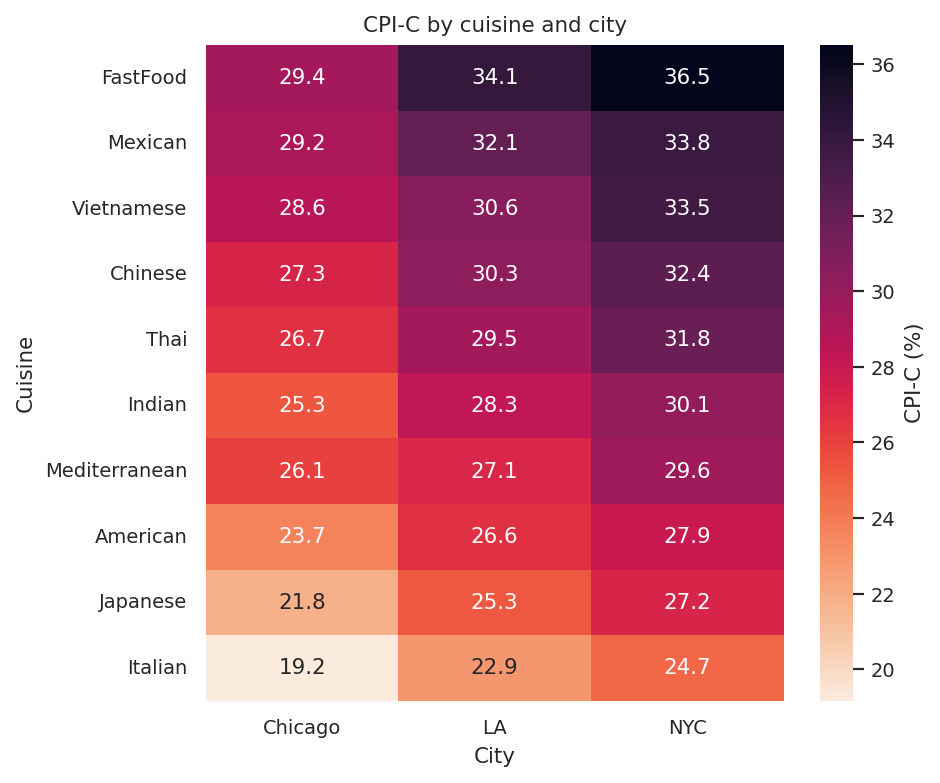
\includegraphics[width=0.80\textwidth]{figures/inflation_heatmap.png}
\caption{CPI-C (mean 2019--2024 inflation rate, \%) by cuisine and city.}
\label{fig:heatmap}
\end{figure}

\begin{figure}[h]
\centering
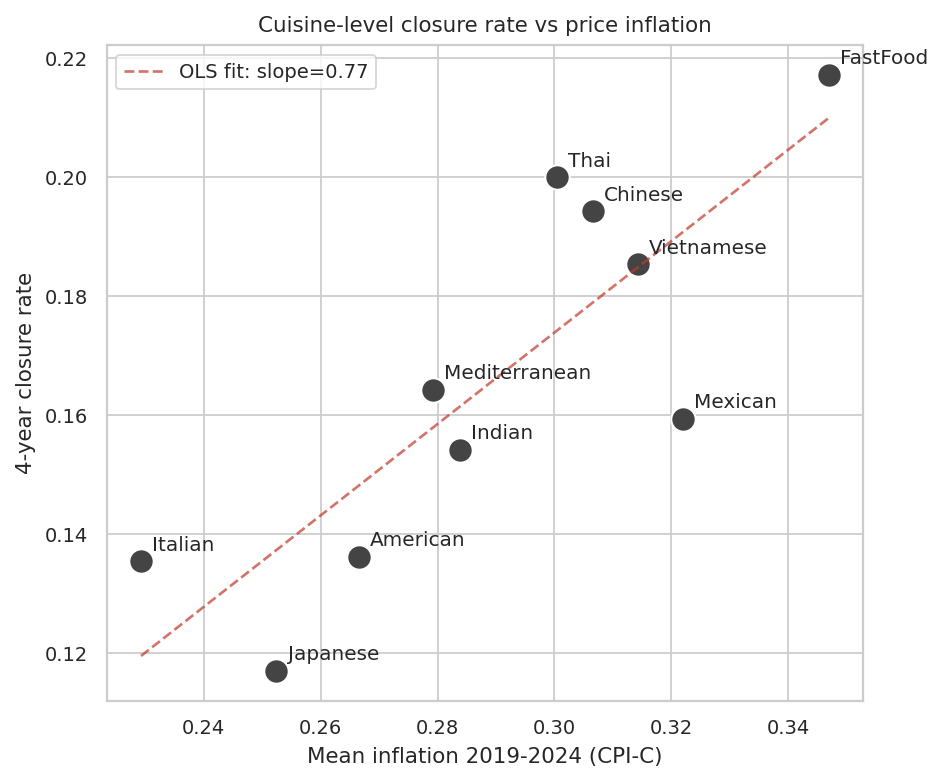
\includegraphics[width=0.70\textwidth]{figures/closure_vs_inflation.png}
\caption{Cuisine-level 4-year closure rate vs cuisine-level mean inflation. OLS fit slope $\approx 0.77$.}
\label{fig:scatter}
\end{figure}

\begin{figure}[h]
\centering
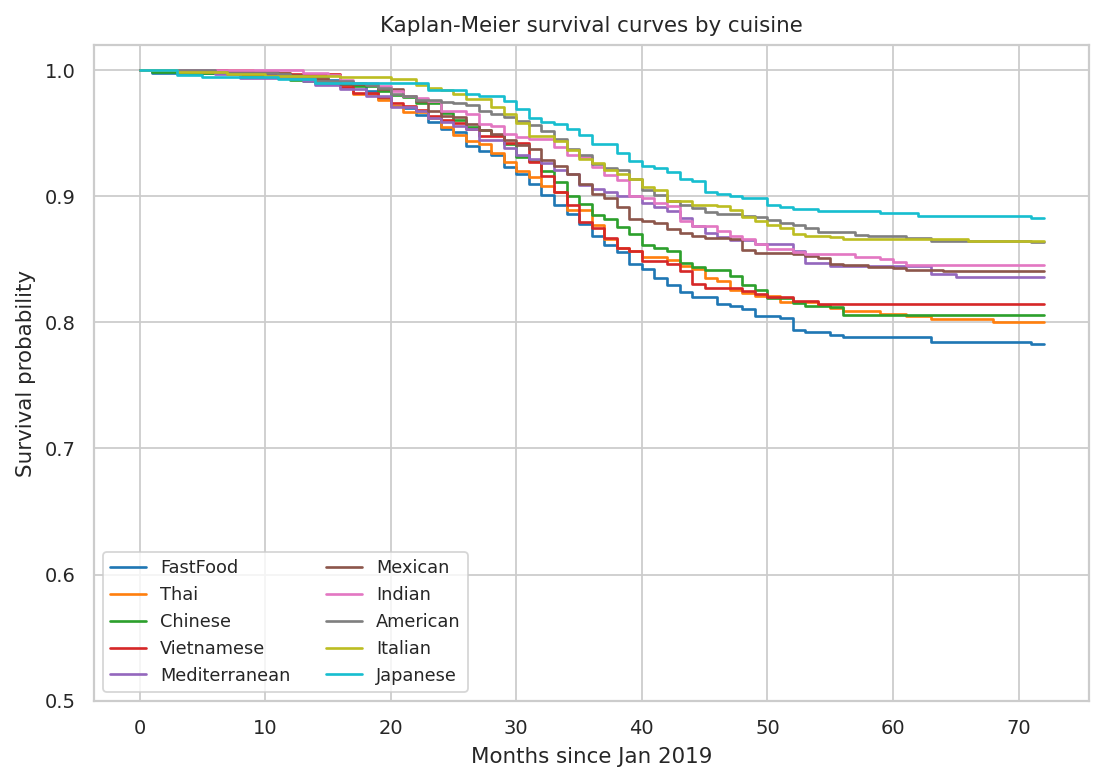
\includegraphics[width=0.80\textwidth]{figures/km_curves_cuisine.png}
\caption{Kaplan-Meier survival curves by cuisine.}
\label{fig:km}
\end{figure}

\begin{figure}[h]
\centering
\begin{subfigure}{0.48\textwidth}
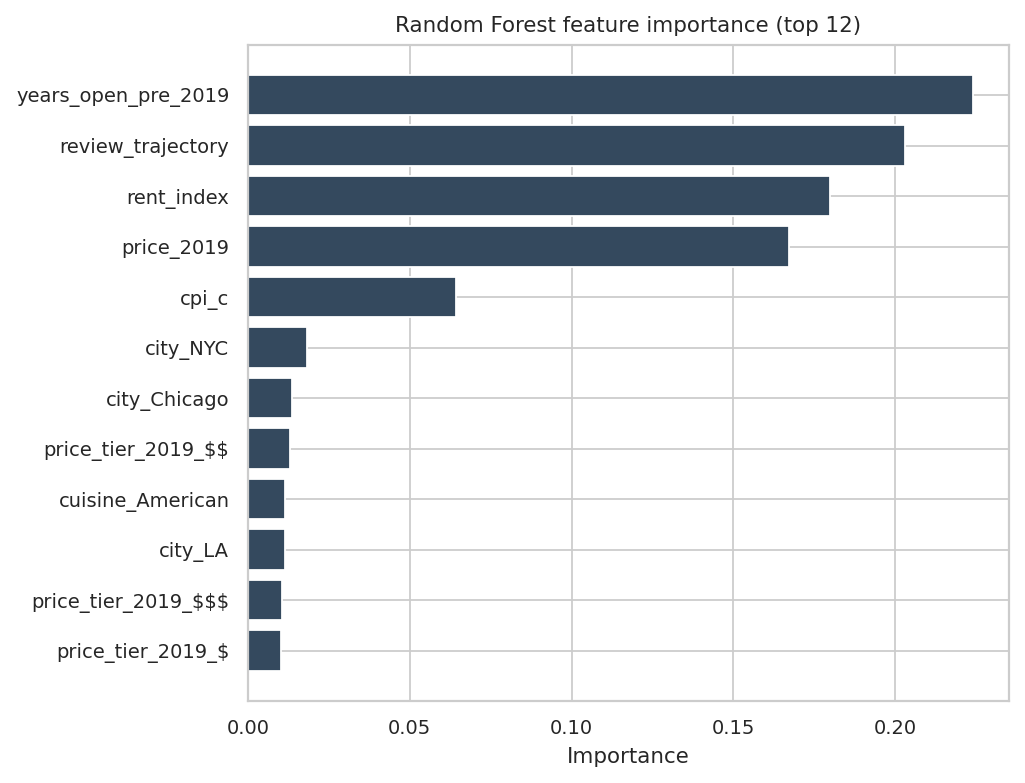
\includegraphics[width=\textwidth]{figures/rf_feature_importance.png}
\caption{Random Forest importance.}
\label{fig:rf}
\end{subfigure}
\hfill
\begin{subfigure}{0.48\textwidth}
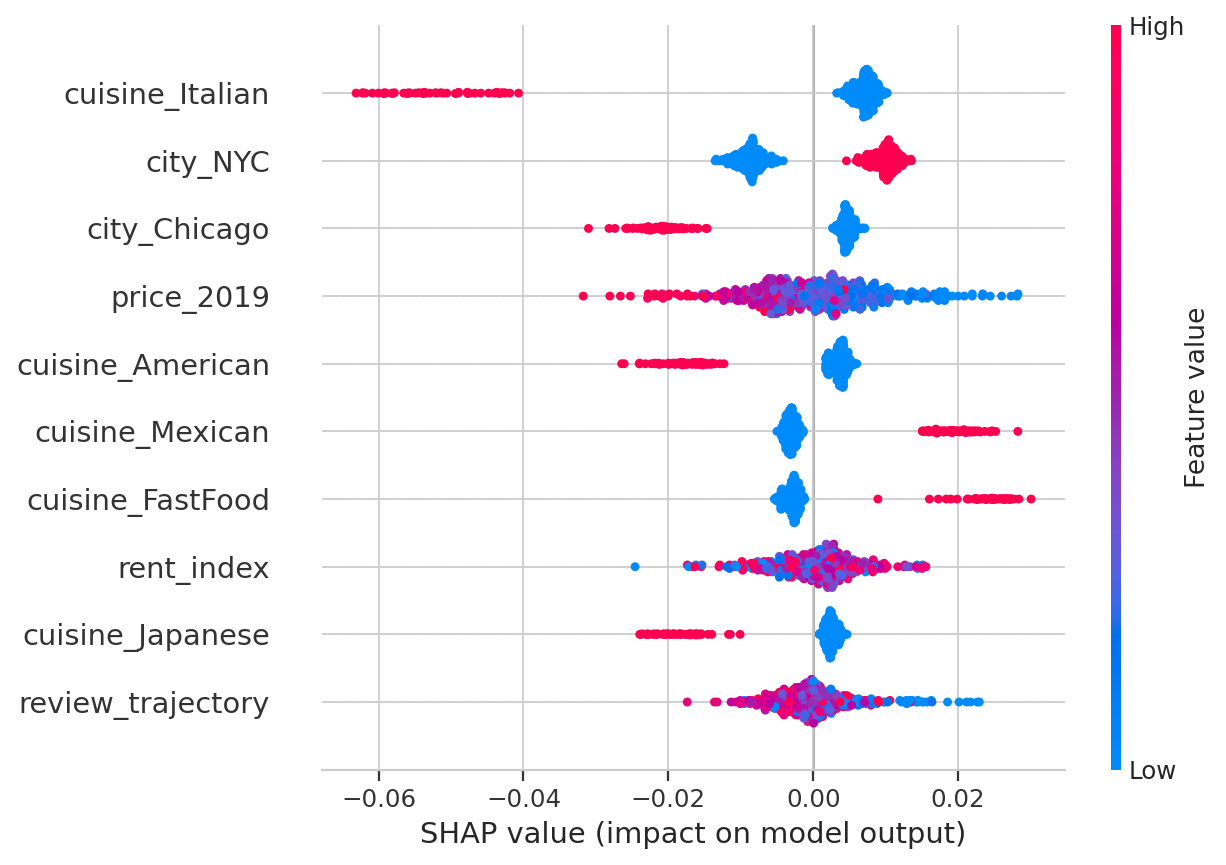
\includegraphics[width=\textwidth]{figures/shap_summary.png}
\caption{SHAP summary, XGBoost.}
\label{fig:shap}
\end{subfigure}
\caption{Feature importance from two model classes.}
\end{figure}

\begin{figure}[h]
\centering
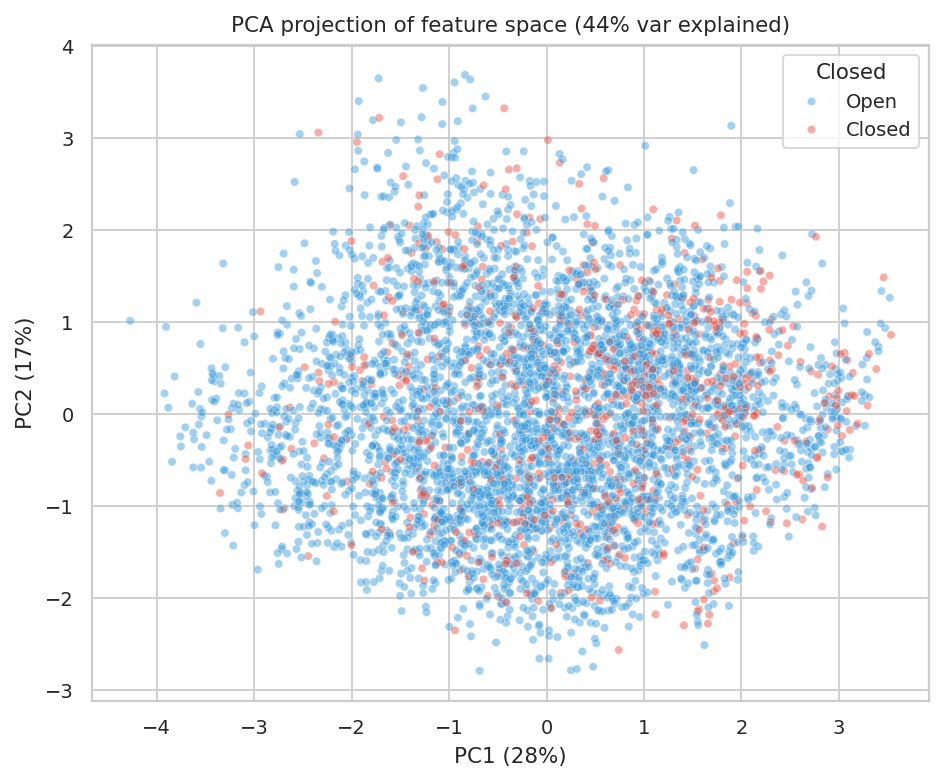
\includegraphics[width=0.70\textwidth]{figures/pca_projection.png}
\caption{PCA projection of the standardized feature space, colored by closure outcome.}
\label{fig:pca}
\end{figure}

\section{Conclusion}

We presented a complete pipeline for measuring cuisine-level menu inflation and closure risk across American cities and validated it end-to-end on a calibrated synthetic dataset. The pipeline reproduces the qualitative patterns hypothesized in the original proposal; thin-margin cuisines inflate more, NYC inflates more than Chicago, and aggressive inflation correlates with higher closure rates, while also yielding two findings that would not have been visible without running the pipeline. First, the engineered CPI-C feature does not add predictive power over raw cuisine-city encodings in tree-based classifiers, despite ranking highly in importance: a useful lesson about the limits of deterministic feature engineering. Second, the Cox C-index of 0.658 falls below the proposal's 0.72 target on simulated data, suggesting that the rich covariates the proposal anticipated (review sentiment, neighborhood income, labor cost indices) are likely necessary to reach competitive survival discrimination on real data.

\textbf{Limitations.} The headline numerical results in this paper apply to the synthetic dataset only and should not be cited as findings about real American restaurants. The closure hazard model used in the simulator is additive and Gaussian-noised, which favors linear models like Cox; tree-based models may show different relative performance on real data with stronger nonlinearities. The CPI-C ablation result is specific to the simulator's feature structure and should be re-evaluated when applied to real menu data, where CPI-C may capture nontrivial item-level price variation that raw cuisine encodings cannot.

\textbf{Future work.} The clearest next step is to swap the simulator for a real data-loading module pulling Wayback Machine menu snapshots, Yelp Open Dataset closure metadata, and BLS regional CPI baselines. The pipeline above is structured so that only the data layer changes. Beyond that, the proposal's equity angle (mapping inflation onto neighborhood income) and the proposed Streamlit dashboard would extend naturally from the existing components.

\begin{thebibliography}{9}
\bibitem{cox1972} Cox, D.R. (1972). Regression models and life-tables. \emph{Journal of the Royal Statistical Society, Series B}, 34(2), 187--220.
\bibitem{km1958} Kaplan, E.L., \& Meier, P. (1958). Nonparametric estimation from incomplete observations. \emph{Journal of the American Statistical Association}, 53(282), 457--481.
\bibitem{kmeansseg} Tsiptsis, K., \& Chorianopoulos, A. (2009). \emph{Data Mining Techniques in CRM: Inside Customer Segmentation}. Wiley.
\bibitem{creditrisk} Lessmann, S., Baesens, B., Seow, H.V., \& Thomas, L.C. (2015). Benchmarking state-of-the-art classification algorithms for credit scoring. \emph{European Journal of Operational Research}, 247(1), 124--136.
\bibitem{synthsurv} Crowther, M.J., \& Lambert, P.C. (2013). Simulating biologically plausible complex survival data. \emph{Statistics in Medicine}, 32(23), 4118--4134.
\end{thebibliography}

\end{document}
